% !TeX root = ../thuthesis-example.tex

\begin{translation}
\label{cha:translation}

\title{车队的队列稳定性:定义和分析方法}
\maketitle

% \tableofcontents

  \vspace{1em}
  \textbf{摘要:}由互相关联的自动驾驶车辆 (connected and automated vehicles, CAVs) 组成的车队预计将对道路交通产生变革性影响,例如提高高速公路安全性、提高交通效率和减少燃料消耗。控制车队时的一项关键任务是实现队列稳定性(String Stability),
  为此提出了许多模型和算法。但是,尽管这些年来针对队列稳定性提出了许多不同的定义和分析方法,但是没有进行详尽的比较。 为了填补这些空白,本文旨在阐明这些模糊的定义与各种分析方法之间的关系,为今后的研究提供一个坚实
  的基础。本文总结和讨论了一系列等价的定义和算法,也讨论了不同分析方法和定义的优、缺点。 所有这些讨论为在实际使用中选择车队的分析方法提供了见解。

\section{引言}

  作为一种提高交通效率的有效方式,车队控制引起了广泛的兴趣。(Guanetti, Kim, and Borrelli, 2018; Horowitz and Varaiya, 2000; Ioannou and Chien,1993; Li, Zheng, Li, and Wang, 2015; Sheikholeslam and Desoer, 1990; Shladover, 1995)
  在一个车队中,由两辆及以上车辆组成的车队按照预先设置的巡航速度和车间距行驶。与人工驾驶相比,自动驾驶车队有着车与车之间的距离更小的优点(即队形更加紧密),被认为是一个很有希望的降低交通阻塞、空气阻力和燃油损耗的方法。
  (Al Alam, Gattami, and Johansson, 2010; Chien and Ioannou, 1992; Liand Chen, 2017)
  
  车队的紧密编队控制有一个特殊的困难,称为“队列不稳定性”,即系统中的扰动沿着车队不断放大,如图~\ref{fig:appendix-translation-figure1}(b)所示(参见Peppard(1974))。 
  正如观察 (Treiterer and Myers, 1974) 和实验 (Sugiyama et al., 2008) 所证明的那样,紧密编队车队的队列不稳定性会导致在环形线路和高速公路上出现没有瓶颈的堵塞(例如,走走停停),这严重损害了车队控制的好处。

\begin{figure}
  \centering
  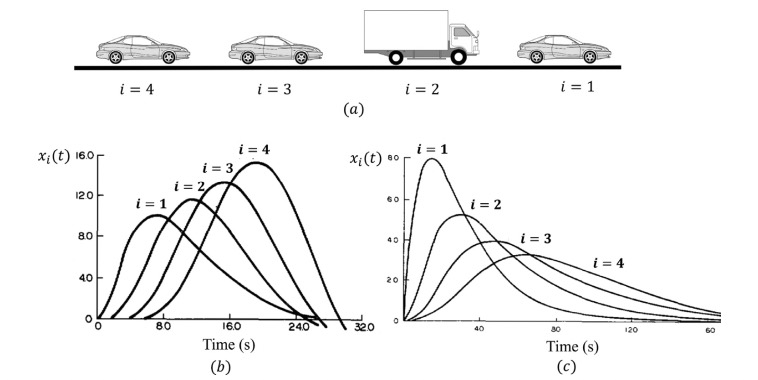
\includegraphics[width=1\linewidth]{appendix-A-1.jpg}
  \caption{车队系统图示(a)和队列稳定性的直观描述(b-c)(Peppard, 1974),其中$x_i(t)$表示车辆$i$在时间$t$的状态波动(例如位置误差)。}
  \label{fig:appendix-translation-figure1}
\end{figure}
   
  为了解决这个问题,队列稳定性的性质已经被广泛研究并应用于车队控制。直观地说,如果一个车队具有以下特性,则称它是队列稳定的,即扰动不会沿着车队被不断放大(Peppard,1974),
  如图~\ref{fig:appendix-translation-figure1}(c)所示。研究队列稳定性的基本过程可分为三个步骤:(1)数学上定义队列稳定性的性质;(2)根据分析方法推导出充分条件;(3) 设计控制器以满足充分条件

\subsection{研究动机}

  大量文献提出了很多种不同的的定义和分析方法。在许多研究中,虽然仿真结果显示出与图~\ref{fig:appendix-translation-figure1}(c)相似的性质,但队列稳定性的性质存在令人困惑的差异。
  许多不同的定义是基于不同的域(例如频域和时域)和范数(例如$\mathcal{L_2}$、$\mathcal{L_p}$和$\mathcal{L_\infty}$)、强度(例如弱和强)。模棱两可的定义阻碍了不同研究之间的比较。
  需要对它们之间的关系进行严格的分析以帮助进一步研究的进行。此外,学者已经提出了许多分析方法并衍生了许多性质,它们的关系、利弊以及可以解决什么问题尚未得到太多讨论。
  更好地理解这些方法和性质是进一步研究困难问题的基础。

\subsection{研究范围和目的}

本文重点介绍队列稳定性的定义和推导队列稳定性质的分析方法。为了更好地解释相关概念,我们将简要介绍一些车队控制的研究工作。然而,为了简明扼要,本文将不讨论车队控制领域的其他问题。
(Li et al., 2015; Li, Zheng et al., 2017)。

本文的目的是:(1)阐明队列稳定性模糊定义之间的关系,提出统一的定义; (2)讨论各种分析方法的关系、利弊、可以解决什么问题,并针对存在的棘手问题提出方法建议;(3)深入研究各性质之间的关系,
这为解决队列不稳定的问题提供了思路。

\subsection{主要贡献}

  本工作的主要贡献为:

  第一,严格分析了模糊不清的定义之间的关系。对常用的定义进行了介绍和比较。总结了队列稳定性的三个基本属性,即收敛性、有界性和可扩展性。类似于控制理论中稳定性定义,
  本文提出了三种类型的队列稳定性定义作为不同定义之间的桥梁,即李雅普诺夫稳定性、输入-输出稳定性和输入-状态队列稳定性。定理1详细阐述了对这些队列稳定性定义的严格分析。
  受该定理的启发,建议将所提出的定义,即输入-状态队列稳定性 (ISSS)用于未来的研究。,并且给出了推荐ISSS的理由。本文扩展并深化了对该领域先前主要对定义的讨论。
  (Ploeg, Van De Wouw, and Nijmeijer, 2014; Stüdli, Seron, and Middleton, 2017)

  第二,本文对各种分析方法进行了比较,并对通过使用这些分析方法推导得到的性质进行了严格的分析。这些方法可以分为三类:时间域分析方法、$z$域分析方法和$s$域分析方法。
  带分析的问题可分为时间维度和空间维度。本文分别从两个维度讨论了这些分析方法的优缺点,在此基础上我们推荐了针对现有困难问题的方法。此外,在定理2中对推导得到的性质进行了严格分析,
  从中展现了这些性质以及常用研究队列系统的推荐定义(即ISSS)之间的关系。 并将解决队列不稳定的常用解决方法与“弱耦合性质”进行了比较。

\section{预备知识}
  记实数域为$\mathbb{R}$,自然数集$\mathbb{N}={1, 2, \dots}$,对于向量$\chi \in \mathbb{R}^n$,其$p$范数为
  \begin{equation}
    \Vert\chi\Vert_p = \left( \sum_{i=1}^n{|\chi_i|^p} \right) ^{1/p}, p \in [1, \infty)
    \label{eq:appendix-equation-1}
  \end{equation}
  \begin{equation}
    \Vert\chi\Vert_\infty = \max_{i} |\chi_i|.
    \label{eq:appendix-equation-2}
  \end{equation}
  对于一个勒贝格可测的信号$\chi(t):I \rightarrow \mathbb{R}^n$,其$\mathcal{L}_p$范数$\Vert\chi\Vert^I_{\mathcal{L}_p}$定义为
  \begin{equation}
    \Vert\chi\Vert^I_{\mathcal{L}_p} = \left( \int_I{\Vert\chi\Vert_p^p dt} \right) ^{1/p} < \infty, p \in [1, \infty)
    \label{eq:appendix-equation-3}
  \end{equation}
  \begin{equation}
    \Vert\chi\Vert^I_{\mathcal{L}_\infty} = \sup_{t \in I} \Vert\chi\Vert_\infty,
    \label{eq:appendix-equation-4}
  \end{equation}
  当$I=[0, \infty)]$时,$\Vert\chi\Vert^{[0, \infty)]}_{\mathcal{L}_\infty}$简记为$\Vert\chi\Vert_{\mathcal{L}_\infty}$。给定一个系统的传递函数$G(j\omega)$,系统的$\mathcal{H}_\infty$范数定义为
  \begin{equation}
    \Vert G \Vert_{\mathcal{H}_\infty} = \sup_{\omega}|G(j\omega)|, {\rm (SISO)}
    \label{eq:appendix-equation-5}
  \end{equation}
  \begin{equation}
    \Vert G \Vert_{\mathcal{H}_\infty} = \sup_{\omega}\bar{\sigma} \left( G(j\omega) \right), {\rm (MIMO)}
    \label{eq:appendix-equation-6}
  \end{equation}
  SISO代表单输入单输出系统,MIMO代表多输入多输出系统。$\bar{\sigma} \left( G(j\omega) \right)$是矩阵$G(j\omega)$的最大奇异值(参见Zhou, Doyle, Glover et al., 1996)。
  对于连续函数$\alpha:[0, a) \rightarrow [0, \infty), a \in \mathbb{R}^+$,如果在其定义域上是严格单调递增的,并且$\alpha(0) = 0$,那么我们称这个函数是$\mathcal{K}$类函数。
  对于连续函数$\beta:[0, a) \times [0, \infty) \rightarrow [0, \infty)$,如果对于每一个固定的$s$,函数$\beta(\cdot, s)$是$\mathcal{}$类函数,并且对于每一个固定的$r$,函数$\beta(r, \cdot)$
  在其定义域上是单调递减的,且满足当$s \rightarrow 0$时,$\beta (r, s) \rightarrow 0$,那么我们称这个函数是$\mathcal{KL}$类函数。如果$\Vert\chi\Vert_{\mathcal{L}_\infty} < \infty$,我们
  称$\chi \in \mathcal{L}_\infty$。

  通常,我们考虑一个车队
  \begin{align}
    \dot{\chi} &= f(\chi, \omega), \\
    \label{eq:appendix-equation-7}
    y &= g(\chi)
  \end{align}

  这里,函数$f(\chi, \omega): \mathbb{R}^{mn} \times \mathbb{R}^m \rightarrow \mathbb{R}^{mn}$是连续可导且全局Lipschitz的,
  函数$g(\chi): \mathbb{R}^{mn} \rightarrow \mathbb{R}^{m}$是连续可导且全局Lipschitz的。$\chi \in \mathbb{R}^{mn}$代表系统状态向量,
  $\omega \in \mathbb{R}^m$代表扰动。我们假设原点$\chi = 0$是非受迫系统$\dot{\chi} = f(\chi, 0)$的一个稳定平衡点。对于车队,$m \in \mathbb{N}$
  代表了车队长度,$n \in \mathbb{N}$代表子系统的状态阶数,表\ref{tab:appendix-translation-table1}列出了这些符号的含义。

  \begin{table}
    \centering
    \caption{所用变量的符号}
    \begin{tabular}{ll}
      \toprule
      变量          & 符号                        \\
      \midrule
      $S_m$           & $S_m = \{0\} \cup \{i \in \mathbb{N} | 1 \leqslant i \leqslant m-1 \}.$ \\
      $S_{e,m}$       & $S_m = \{i \in \mathbb{N} | 1 \leqslant i \leqslant m-1 \}.$                     \\
      $\chi_i(t)$     & $\chi_i(t) \in \mathbb{R}^n$代表第$i$个子系统的状态   \\
      $\omega_i(t)$   & $\omega_i(t) \in \mathbb{R}$代表第$i$个子系统受到的扰动 \\
      $y_i(t)$        & $y_i(t) \in \mathbb{R}$代表第$i$个子系统的输出        \\
      $\chi_i(t)$     & $\chi_i(t) \in \mathbb{R}^{mn}$代表系统的状态        \\
      $\omega(t)$     & $\omega(t) \in \mathbb{R}^m$代表系统受到的扰动        \\
      $y(t)$          & $y(t) \in \mathbb{R}^m$代表系统的输出        \\
      $\Chi_i(s), Y_i(s), U_i(s)$   & $\chi_i(t), y_i(t), u_i(t)$的拉普拉斯变换        \\
      $\Chi(s), Y(s), U(s)$         & $\chi(t), y(t), u(t)$的拉普拉斯变换        \\
      $\mathcal{\Chi}(z), \mathcal{Y}(z), \mathcal{U}(z)$   & $\chi(t), y(t), u(t)$的$z$变换        \\
      \bottomrule
    \end{tabular}
    \label{tab:appendix-translation-table1}
  \end{table}


\section{车队控制}

本节简要介绍了车队的控制问题,该问题引发了对队列稳定性的研究。车队的控制问题最初由Levine和Athans于1966年提出,研究如何设计一个控制器来实现队列系统的控制。
这包括队列系统描述、控制目标和控制器设计方法。并且介绍了本文的两个重点的背景,即队列稳定性的定义和分析方法。

\subsection{队列系统描述}

车队系统的描述确定了队列稳定问题的研究场景。本文采用了由四个部分组成的框架(Li et al., 2015),即节点动力学、信息流拓扑结构、分布式控制和构成几何。
此外,还强调了系统的通信质量和收到的干扰。一个特定的车队系统可以通过这六个部分来唯一确定,本小节中用到的缩写在表\ref{tab:appendix-translation-tableA1}中列出。

\subsubsection{节点动力学}

节点动力学(node dynamics, ND)表示车辆在纵向的动力学。根据建模,车辆动力学模型可分为非线性(Dunbar and Caveney, 2012; Rajamani, 2011),
二阶模型(Naus, Vugts, Ploeg, van de Molengraft, and Steinbuch, 2010; Yanakiev and Kanellakopoulos, 1996),
三阶模型(Godbole and Lygeros, 1994; Liang and Peng, 1999; Warnick and Rodriguez, 2000),和一般线性模型(Liang and Peng, 2000; Seiler, Pant, and Hedrick, 2004)。

\subsubsection{信息流拓扑结构}

信息流拓扑结构(information flow topology, IFT)描述了车辆如何与其他车辆交换信息。图\ref{fig:appendix-translation-figure2}所示为常用的拓扑结构,包括前继跟随拓扑(PF)(Naus et al., 2010)、
前继领导跟随拓扑(PLF)(Sheikholeslam and Desoer, 1990; Swaroop and Hedrick, 1999)、
双向拓扑(BD)(Eyre, Yanakiev, and Kanellakopoulos, 1997; Ghasemi, Kazemi, and Azadi, 2013; Knorn, Donaire, Agüero, and Middleton, 2014; Yanakiev and Kanellakopoulos, 1996),
双向领导拓扑(BDL)(Zheng, Li, Wang, Cao, and Li, 2016),
双前继跟随拓扑(TPF)(Swaroop and Hedrick, 1999),
以及双前继领导跟随拓扑(TPLF)(Li et al., 2015)。
也可以应用更一般的信息流拓扑结构,例如,$r$前继跟随拓扑($r$PF)和$r$前继领导跟随拓扑($r$PLF),其中$r$表示有之交流的前继数量。

\begin{figure}
  \centering
  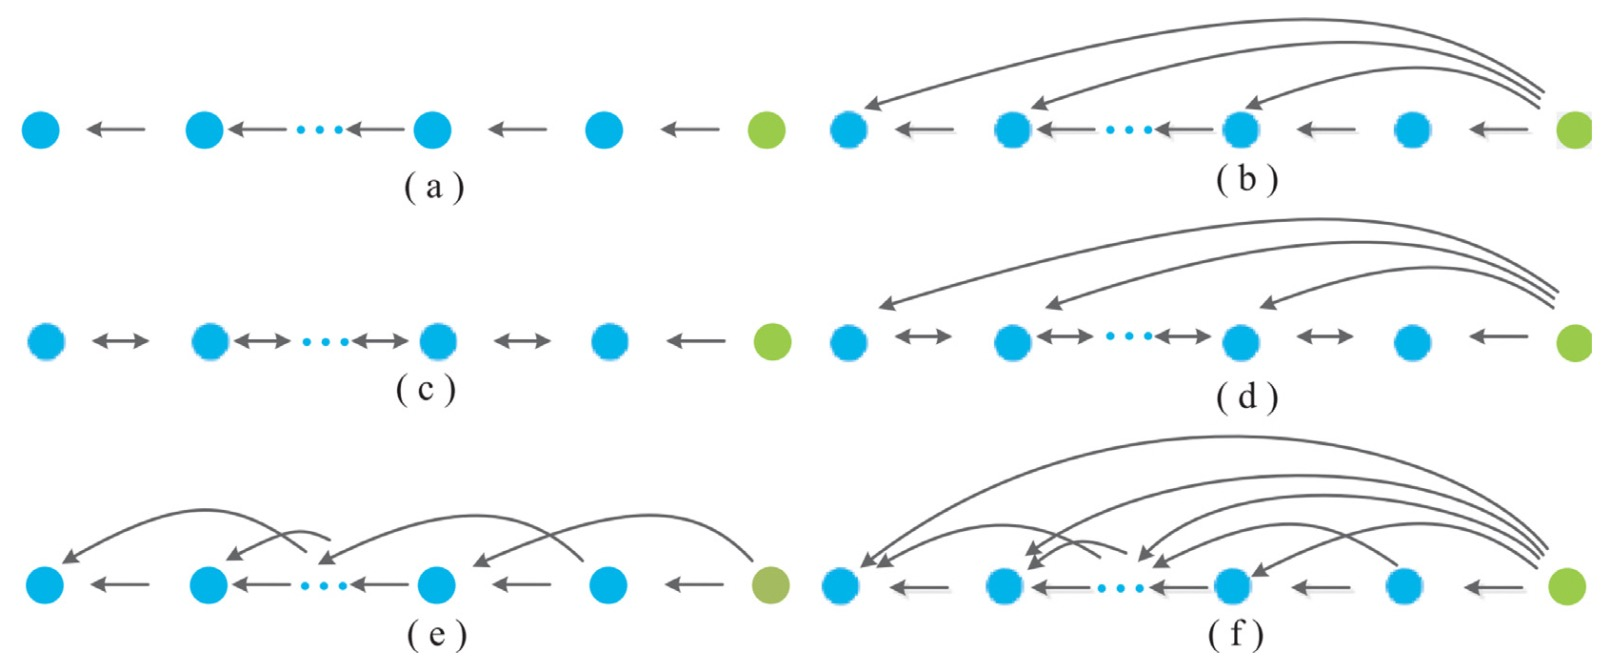
\includegraphics[width=1\linewidth]{appendix-A-2.jpg}
  \caption{车队的的典型信息流拓扑结构,其中绿色圆圈表示头车。(a)PF;(b)PLF;(c)BD;(d)BDL;(e)TPF;(f)TPLF(Li et al., 2015)。}
  \label{fig:appendix-translation-figure2}
\end{figure}

\subsubsection{分布式控制器}

分布式控制器(distributed controller, DC)描述了用于实现控制目标的对车队系统的控制器,例如,线性控制器(Nauset al.,2010;Sheikholeslam and Desoer,1993)、
最优控制器(Chu,1974b;Jin and Orosz,2017;Liang and Peng,1999)、$H_\infty$控制器(Ploeg, Shukla, van de Wouw, and Nijmeijer,2014)、
模型预测控制(MPC)(Dolk, Ploeg, and Heemels, 2017; Dunbar and Caveney, 2012),以及滑模控制(SMC)(Fernandes and Nunes,2012)。

\subsubsection{构成几何}

车队的构成几何(formation geometry, FG)表示车队所期望的车辆间距离,在许多研究中也被称为间距策略。现在存在三种主要政策,
即恒定距离(constant distance, CD)政策(Liu, Goldsmith, Mahal., and Hedrick, 2001; Sheikholeslam and Desoer, 1993)、
恒定时间间隔( constant time headway, CTH)政策(Chien and Ioannou, 1992; Zhou and Peng, 2005),
以及非线性距离(nonliear distance, NLD)政策(Orosz, 2016; Santhanakrishnan abd Rajamani, 2003)。

\subsubsection{通信质量}

通信质量(communication quality, CQ)描述了由其引起的问题,即通信时间延迟(di Bernardo, Salvi, and Santini, 2015; Liu et al., 2001; Oncu, Van de Wouw, 
Heemels, and Nijmeijer, 2012; Qin, Gomez, and Orosz, 2017; Xiao, Darbha, and Gao, 2008; Xiao, Gao, and Wang, 2009)
和丢包(Moreau, 2005; Ploeg, Semsar-Kazerooni, Lijster, van de Wouw, and Nijmeijer, 2015; Teo, Stipanovic, and Tomlin, 2002; 2003)。

\subsubsection{扰动}

扰动是造成车队系统产生偏差的原因,常用的扰动类型包括:
\begin{itemize}
  \item 第一类:头车的初始条件扰动;
  \item 第二类:所有车辆的初始条件扰动;
  \item 第三类:头车受到的零初始条件外部扰动;
  \item 第四类:所有车辆受到的零初始条件外部扰动。
\end{itemize}


最后,介绍两个车队系统的重要术语,即同质性和无限性。如果所有车辆都具有相同的动力学特性,则称该车队具有同质性(Chu,1974a);否则称其具有异质性(Naus等,2010)。
此外,如果车队有无限辆车辆组成,则称其为无限的(Swaroop and Hedrick, 1996);否则称为有限的(Jin and Orosz, 2014)。
理论分析使得研究人员可以通常研究无限车队,以研究由大量但有限辆车组成的车队的本质(Curtain, Iftime, and Zwart, 2010; Jovanovic and Bamieh, 2005)和车队的可扩展性。

\subsection{控制目标}

控制自动驾驶车辆车队的目的是确保同一组的所有车辆以一致的速度移动,同时相邻车辆之间保持理想距离,从而提高交通容量,改善交通安全性,并减少燃料消耗(Horowitz and Varaiya, 2000)。
车队系统的稳定性特性是上述所有控制目标的基础。研究人员已经提出了两种类型的稳定性,个体稳定性和队列稳定性。

个体稳定性描述了车辆向给定轨迹收敛的情况(Dolk et al., 2017; Dunbar and Caveney, 2012; Ghasemi et al.,2013; Guo, Ding, and Han, 2014; Ploeg,Shukla et al., 2014; Swaroop and Hedrick, 1999; Zheng, Li, Wang et al., 2016),
收敛速度由稳定系数描述(Barooah, Mehta, and Hespanha, 2009; Hao and Barooah, 2012; Hao, Barooah, and Mehta, 2011; Zheng, Li, Li, and Wang, 2016)。
然而,随着长度的增加,一个每个个体都稳定的车队仍然可能将一个小的扰动放大并造成交通拥堵(例如走走停停)(Hedrick, Tomizuka, and Varaiya, 1994; Naus et al., 2010。 Shaw and Hedrick, 2007b; Sugiyama et al., 2008)。

为了解决这个问题,研究人员提出了队列稳定性并对其做了大量研究。直观地说,如果扰动在沿车队向下游传播时不被放大,那么就可以说车队是队列稳定的(Peppard, 1974)。
为了从数学上定义这一特性,在过去的几十年里,针对不同的车队系统提出了各种正式的队列稳定定义,例如(Jin and Orosz, 2014; Khatir and Davidson, 2004; Li, Shi, and Yan, 2016; Ploeg,Van De Wouw et al., 2014; Swaroop and Hedrick, 1996)。
这些定义的详细情况将在下一节讨论,它们之间的关系是本文的一个重点。

\subsection{控制器设计方法}

设计一个车队控制器的关键是要实现控制目标,如个体稳定性和队列稳定性。

一类最常用的设计方法是预先确定一个反馈控制器并调整其参数以实现控制目标。数学上,实现队列稳定性被重新定义为传递函数需要满足的的某些条件(Jin and Orosz, 2014; Naus et al., 2010; Orosz, 2016),
或李雅普诺夫函数(Besselink and Johansson, 2017; Dolk et al., 2017; Swaroop and Hedrick, 1996)。这些方法的共同局限性是难以明确地满足饱和约束,如输入饱和和安全约束。

另一类设计方法是前馈控制(Li and Li, 2019; Liu, Li, Li, and Wang, 2017),例如分散模型预测控制(decentralized model predictive control, DMPC)方法(Dunbar and Caveney, 2012)。
个体稳定性和队列稳定性的性质被显式约束。通过解决每个控制环节中的优化问题,控制器可以保证实现控制目标。

这两类方法的关键步骤是分析队列稳定性质并推导出其充分条件。如果所设计的控制器满足其充分条件,则系统必然是队列稳定的。因此,队列稳定性质的分析方法是非常关键的,也是本文的另一个重点。

\section{队列稳定性定义}

本节介绍了车队控制问题中常用的队列稳定性的定义。队列稳定性定义的发展与车队系统的相关假设密切相关,并深深影响着分析方法。因此,在介绍一个新的定义时,将简要讨论具体的车队系统和分析方法。定义的缩写见表\ref{tab:appendix-translation-tableA2}。

\subsection{队列稳定原始定义(OSS)}

我们首先回顾Chu(1974a)给出的队列稳定(original definition of string stability, OSS)的原始定义。

\begin{definition}[OSS]
  如果对于车队中的所有车辆,在初始时受到任意一组有界的扰动,所有车辆的位置波动保持有界,并且这些波动在$t \rightarrow 0$时是趋于0的,那么这个车队是稳定的。
  \label{def:appendix-translation-def1}
\end{definition}

如果受到的是有界的第一类或第二类干扰,定义\ref{def:appendix-translation-def1}(OSS)呈现了两个性质:

\begin{itemize}
  \item 所有车辆位置波动的有界性;
  \item 所有车辆位置波动的收敛性。
\end{itemize}

为了使有界性非平凡,其应该在车队有任何数量车辆的情况下均成立,即:

\begin{itemize}
  \item 有界性对于任意长度的车队均成立。
\end{itemize}

任意车队长度下的界限不变性是一个重要的性质,它保证了队列稳定性的概念是可扩展的,并且说明了从车队中增加或减少车辆是不影响稳定性的。在某些情况下,收敛性也被称为个体稳定性。
OSS非常接近于对队列稳定性的直观描述(Peppard, 1974),只是位置波动不一定比受到的初始扰动小。位置波动可以被类推到其他系统状态的波动,例如速度。
OSS的主要局限是在理论上不一定对一般车队系统可行。Chu(1974a)提出的$z$变换方法只能用于具有同质ND、IFT、DC、FG和CQ的车队。

\subsection{SFSS与其变体FSS、ESS、HTS}

为了理论分析的方便,Peppard (1974)提出了一个队列稳定在频域下的必要条件,这个条件在之后对队列稳定的研究中得到了广泛的应用,通常被认为是强弦稳定性的定义(Naus et al., 2010)。
因此,我们把这个条件作为频域的强队列稳定(strong frequency-domain string stability, SFSS)的定义来介绍。

\begin{definition}[SFSS]
  对于具有PF拓扑结构的线性车队系统,我们称系统是频域的强队列稳定的(SFSS),如果第$i$辆车和其前车,即第$i-1$辆车,之间的输出传递函数,记作$G_{i-1,i}$,使得
  \begin{equation}
    \Vert G_{i-1,i}(j\omega) \Vert_{\mathcal{H}_\infty} \leqslant 1, \forall i \in S_{e, m}, \forall m \in \mathbb{N}.
    \label{eq:appendix-equation-8}
  \end{equation}
  \label{def:appendix-translation-def2}
\end{definition}
SFSS的一个具体限制是关于车队系统的PF假设。SFSS对于具有其他信息流拓扑结构的车队没有意义,例如对于BD,公式\ref{eq:appendix-equation-8}需要修改(Peppard, 1974)。
对于$r$PF和$r$PLF拓扑结构,人们提出了三个修改的定义,即频域队列稳定(frequency-domain string stability, FSS)(Naus et al., 2010),
终态队列稳定(eventual string stability, ESS)(Khatir and Davidson, 2004),以及队首-队尾稳定(head-to-tail stability, HTS)(Jin and Orosz, 2014; 2017)。

\begin{definition}[FSS]
  对于具有$r$PF或$r$PLF拓扑结构的线性车队系统,我们称系统是频域队列稳定的(FSS),如果头车$0$和任何其他车辆$i$之间的输出传递函数,记为$G_{0, i}$,使得
  \begin{equation}
    \Vert G_{0,i}(j\omega) \Vert_{\mathcal{H}_\infty} \leqslant 1, \forall i \in S_{e, m}, \forall m \in \mathbb{N}.
    \label{eq:appendix-equation-9}
  \end{equation}
  \label{def:appendix-translation-def3}
\end{definition}

\begin{definition}[ESS]
  对于具有$r$PF或$r$PLF拓扑结构的线性车队系统,我们称系统是末态队列稳定的(ESS),如果头车$0$和任何其他车辆$i$之间的输出传递函数,记为$G_{0, m}$,并且存在$N < m$,使得
  \begin{equation}
    \Vert G_{0,i}(j\omega) \Vert_{\mathcal{H}_\infty} \leqslant 1, \forall i > N, \forall m \in \mathbb{N}.
    \label{eq:appendix-equation-10}
  \end{equation}
  \label{def:appendix-translation-def4}
\end{definition}

\begin{definition}[HTS]
  对于具有$r$PF或$r$PLF拓扑结构的线性车队系统,我们称系统是队首-队尾稳定的(HTS),如果头车$0$和任何其他车辆$i$之间的输出传递函数,记为$G_{0, i}$,并且存在$N < m$,使得
  \begin{equation}
    \Vert G_{0,m}(j\omega) \Vert_{\mathcal{H}_\infty} \leqslant 1, \forall m \in \mathbb{N}.
    \label{eq:appendix-equation-11}
  \end{equation}
  \label{def:appendix-translation-def5}
\end{definition}

FSS、ESS和HTS都假定在车队中存在一个头车,这与实际情况是相符的。FSS有时被称为弱队列稳定性,与SFSS相比,它在适用于更多的信息流拓扑结构。ESS是FSS的一个特例,也就是说,
如果一个系统是FSS的,那么它也是ESS的。HTS最初是为混合交通设计的,在混合交通中相互通信的自动驾驶车辆一般在车队尾部(Jin and Orosz, 2014; 2017)。

这些在频域中的定义的第一个局限性是其对车队系统的线性假设。这并不意味着节点动力被假设是线性的,但可以通过适当的非线性反馈方法使其近似线性,例如Sheikholeslam和Desoer(1993),
Stankovic、Stanojevic和Siljak(2000),Ghasemi等人(2013),Zheng、Li、Wang等人(2016)的工作,这需要对车辆动力学有很好的先验知识。

这些定义的第二个局限性是只考虑车队收到了第三类扰动。这个局限性产生于这些定义中拉普拉斯变换时用到的零初始条件假设。其他扰动类型的系统特性需要进一步分析。

第三个也是更关键的局限性是,$\Vert G_{0,m}(j\omega) \Vert_{\mathcal{H}_\infty} \leqslant 1$只能从能量
(即$\mathcal{L}_2$范数)的角度来描述信号,而不是它们的最大振幅(即$\mathcal{L}_\infty$范数)。其详细差异将在下一节讨论。

\subsection{TSS和ATSS}

将队列稳定性的概念推广到一类相互连接的系统中,如

\begin{equation}
  \dot{\chi}_i = f_i(\chi_i, \chi_{i-1}, \cdots, \chi_{i-r}),
  \label{eq:appendix-equation-12}
\end{equation}
其中,$i \in \mathbb{N}$,$\chi \in \mathbb{R}^n$,$\chi_{i-j} \equiv 0, \forall i \leqslant j$,并且$f(0, \cdots, 0) = 0$,
Swaroop和Hedrick(1996)提出了时域队列稳定(time-domain string stability, TSS)和时域渐进队列稳定(asymptotically time-domain string stability, ATSS)。

\begin{definition}[TSS]
  \ref{eq:appendix-equation-12}的原点$\chi_i = 0, i \in \mathbb{N}$是TSS的,如果给定任何$\epsilon > 0$,存在一个$\delta > 0$,使得
  \begin{equation}
    \sup_{i}{|\chi_i(0)|} < \delta \Rightarrow \sup_{i}{\Vert \chi_i(t) \Vert_\infty} < \epsilon.
    \label{eq:appendix-equation-13}
  \end{equation}
  \label{def:appendix-translation-def6}
\end{definition}

\begin{definition}[ATSS]
  \ref{eq:appendix-equation-12}的原点$\chi_i = 0, i \in \mathbb{N}$是ATSS的,如果其是TSS的且渐近地$\sup_{i}{\Vert \chi_i(t) \Vert_\infty} \rightarrow 0$。
  \label{def:appendix-translation-def7}
\end{definition}

\appendix

\section{缩写表}

\begin{table}
  \centering
  \caption{对车队系统的描述的缩写}
  \begin{tabular}{llll}
    \toprule
    缩写       &  全称           &  缩写       &  全称            \\
    \midrule
    ND        &  节点动力学      &  IFT        &  信息流拓扑结构    \\
    PF        &  前继跟随拓扑     &  PLF        &  前继领导跟随拓扑  \\
    BD        &  双向拓扑        &  BDL        &  双向领导拓扑     \\
    TPF       &  双前继跟随拓扑   &  TPLF       &  双前继领导跟随拓扑 \\
    $r$PF     &  $r$前继跟随拓扑  &  $r$PLF     &  $r$前继领导跟随拓扑 \\
    DC        &  分布式控制器     &  MPC        &  模型预测控制       \\
    SMC       &  滑膜控制        &  FG         &  构成几何           \\
    CD        &  恒距            &  CTH       &  恒定车头时距       \\
    NLD       &  非线性距离       &  CQ        &  通信质量          \\
    \bottomrule
  \end{tabular}
  \label{tab:appendix-translation-tableA1}
\end{table}

\begin{table}
  \centering
  \caption{队列稳定定义的缩写}
  \begin{tabular}{llll}
    \toprule
    缩写       &  全称                &   定义       \\
    \midrule
    OSS       &  队列稳定原始定义              &  1           \\
    SFSS      &  频域的强队列稳定              &  2           \\
    FSS       &  频域队列稳定                 &  3           \\
    ESS       &  末态队列稳定                 &  4           \\
    HTS       &  队首-队尾稳定                &  5           \\
    TSS       &  时域队列稳定                 &  6           \\
    ATSS      &  时域渐进队列稳定              &  7           \\
    LPSS      &  $\mathcal{L}_p$队列稳定     &  8           \\
    SLPSS     &  严格$\mathcal{L}_p$队列稳定  &  9           \\
    DSS       &  扰动队列稳定                 &  10          \\
    LSS       &  李雅普诺夫队列稳定            &  11          \\
    ALSS      &  渐进李雅普诺夫队列稳定        &  12          \\
    IOSS      &  输入-输出队列稳定            &  13          \\
    ISSS      &  输入-状态队列稳定            &  14          \\
    \bottomrule
  \end{tabular}
  \label{tab:appendix-translation-tableA2}
\end{table}

% 书面翻译对应的原文索引
\begin{translation-index}
  \nocite{FENG201981}
  \bibliographystyle{unsrtnat}
  \bibliography{ref/appendix}
\end{translation-index}

\end{translation}
